L'infrastruttura di comunicazione consiste tipicamente di sistemi SCADA con canali di comunicazione dedicati da e verso il centro di controllo del sistema e di una Wide Area Network (WAN). I sistemi SCADA collegano tutte le principali strutture operative del sistema mentre la WAN è prevalentemente usata per azioni di mercato. Uno sviluppo importante per la Smart Grid (vedi Figura \ref{fig:cisg}) è quello di estendere la comunicazione a tutto il sistema di distribuzione e di stabilire una comunicazione bidirezionale con i clienti attraverso le Neighbourhood Area Network (NANs) che coprono le zone servite dalle sottostazioni di distribuzione. I clienti avranno la necessità di una Home Area Network (HAN) a cui saranno connessi gli smart device.
\begin{figure}[h]
	\centering
	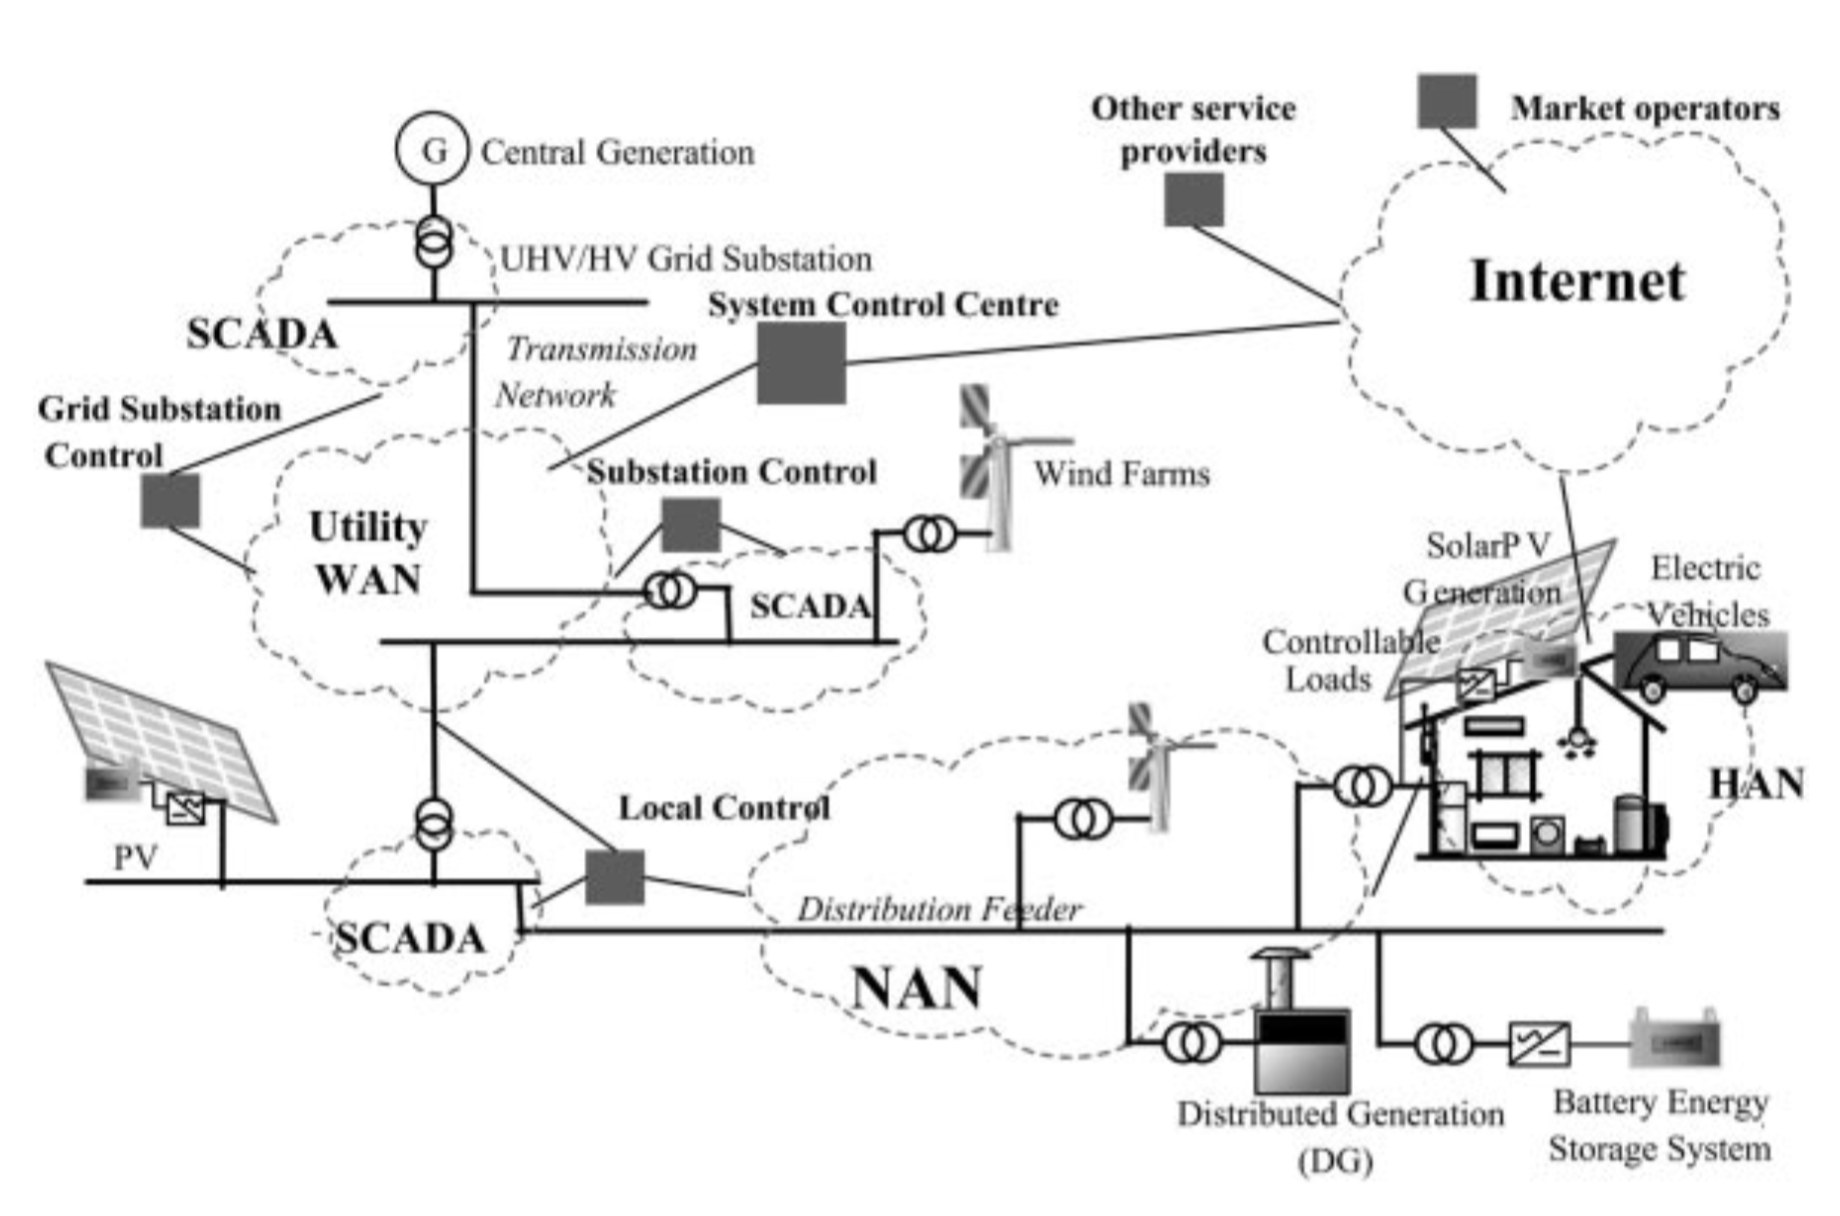
\includegraphics[scale=0.310]{imgs/comm_inf_SG.png}
	\caption{Una possibile infrastruttura di comunicazione per la Smart Grid} \label{fig:cisg}
\end{figure}\\
Le sotto-reti di comunicazione che andranno a comporre la Smart Grid utilizzano diverse tecnologie (vedi Figura \ref{fig:th}) e di particolare interesse è il modo in cui quest'ultime possono essere integrate in maniera efficace. Le Smart Grid possono utilizzare diverse tecnologie di comunicazione wired e wireless (cellulare, satellitare, microwave, WiMAX etc.). Le tecnologie di comunicazione wireless short range, come WiFi e ZigBee,  sono tipicamente utilizzate nelle HAN.
In questo capitolo, saranno descritte alcune tecnologie di comunicazione associate ai livelli inferiori del modello di riferimento ISO/OSI.
\begin{figure}[h]
	\centering
	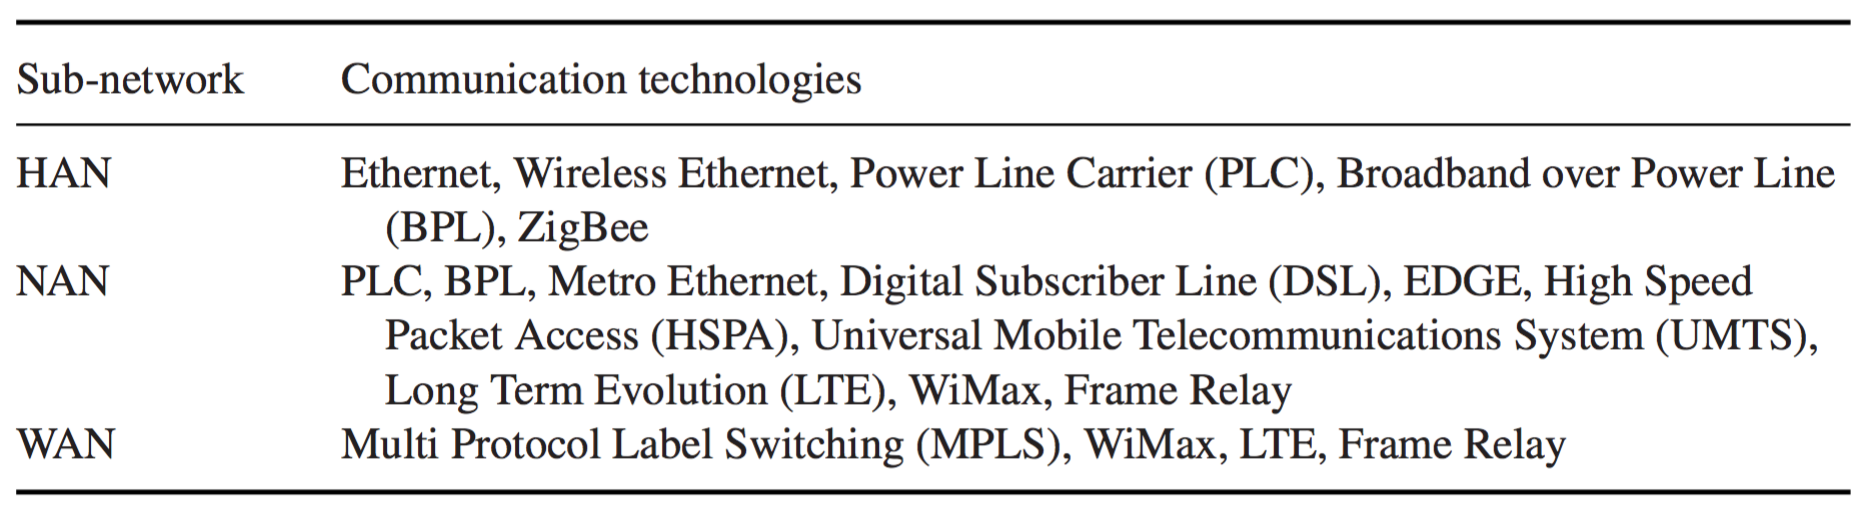
\includegraphics[scale=0.350]{imgs/tech.png}
	\caption{Tecnologie usate nelle differenti sottoreti} \label{fig:th}
\end{figure}

\section{Tecnologie di comunicazione}
\subsection{IEEE 802}
IEEE 802 è una famiglia di standard sviluppati per il supporto alle reti locali (LAN). Facendo riferimento alla Smart Grid, tali standard sono applicabili alle reti LAN in sistemi SCADA, NAN per le reti di distribuzione e HAN nei locali dei clienti. La Figura \ref{fig:arch_802} mostra come l'architettura IEEE 802 è incentrata sui due livelli inferiori del modello ISO/OSI.
\begin{figure}[h]
	\centering
	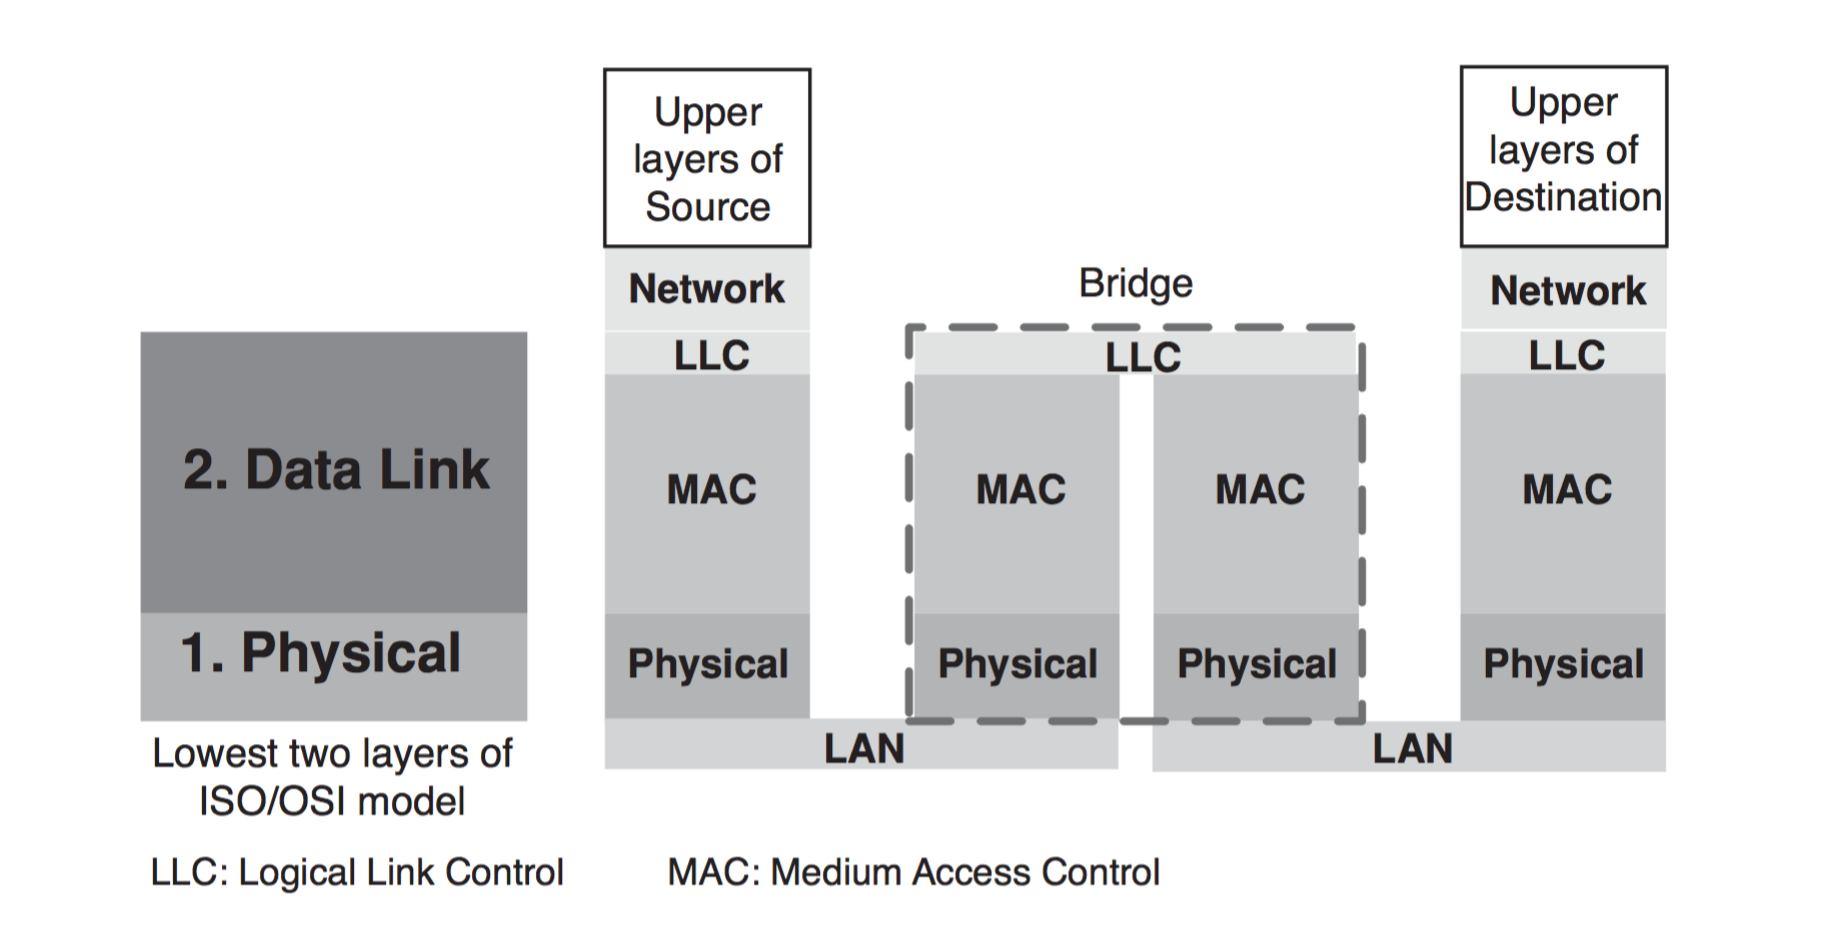
\includegraphics[scale=0.330]{imgs/arch_ieee802.png}
	\caption{Architettura IEEE 802} \label{fig:arch_802}
\end{figure}
Nella Figura in esame è mostrata la connessione di due LAN attraverso l'utilizzo di un Bridge. Tale connessione è comune in molte organizzazioni che hanno più LAN. Un pacchetto dalla sorgente va nel sottostrato Logical Link Control (LLC) che funge da interfaccia tra il livello di rete e il sottostrato MAC. LLC è definito da IEEE 802.2 e fornisce i meccanismi di controllo del flusso, multiplexing e di controllo degli errori. Il pacchetto passa poi nel sottostrato MAC in cui un header ed un trailer vengono aggiunti al pacchetto (a seconda della LAN cui il pacchetto entra). Poi si passa attraverso il livello fisico e nel canale di comunicazione e si raggiunge il Bridge. A livello MAC del Bridge, header e trailer vengono rimossi, recuperando così il pacchetto originale che passa al sottostrato LLC del Bridge. Successivamente il pacchetto viene elaborato dal sottostrato MAC (aggiungendo header e trailer appropriati) in base alla LAN a cui si trasmette. L'utilizzo del Bridge è essenziale in quanto LAN diverse utilizzano differenze dimensioni del frame e velocità (e.g. IEEE 802.3 utilizza un frame di 1500 byte, mentre IEEE 802.4 ne utilizza uno di 8191 byte\cite{802.3}).
\subsubsection{Ethernet}
Ethernet è diventata la tecnologia di rete più utilizzata per le LAN cablate grazie alla sua semplicità, affidabilità, facilità di manutenzione e la capacità di integrare nuove tecnologie. Essa ha un basso costo di installazione ed è facile farne l'upgrade. Si tratta di una tecnologia di comunicazione frame-based che si basa sullo standard IEEE 802.3. Ethernet utilizza un mezzo condiviso che può portare a collisioni tra i frame trasmessi dai vari host. Il problema delle collisioni è gestito da un protocollo chiamato Carrier Sense Multiple Access/Collision Detect (CSMA/CD). Un set di host connessi ad una rete in modo tale che la trasmissione simultanea da due host nel set porta a collisioni, crea un \emph{dominio di collisione}. Inoltre, le LAN Ethernet trasportano anche frame di broadcast il cui dominio raggiungibile è chiamato \emph{dominio di broadcast}. Le prestazioni della rete, in caso di traffico, sono influenzate dal modo in cui i domini di collisione e di broadcast sono posizionati e pertanto l'idea è quella di isolarli per aumentare le prestazioni della rete. La Figura \ref{fig:lan} mostra tali domini su una tipica LAN Ethernet.\newpage
\begin{figure}[h]
	\centering
	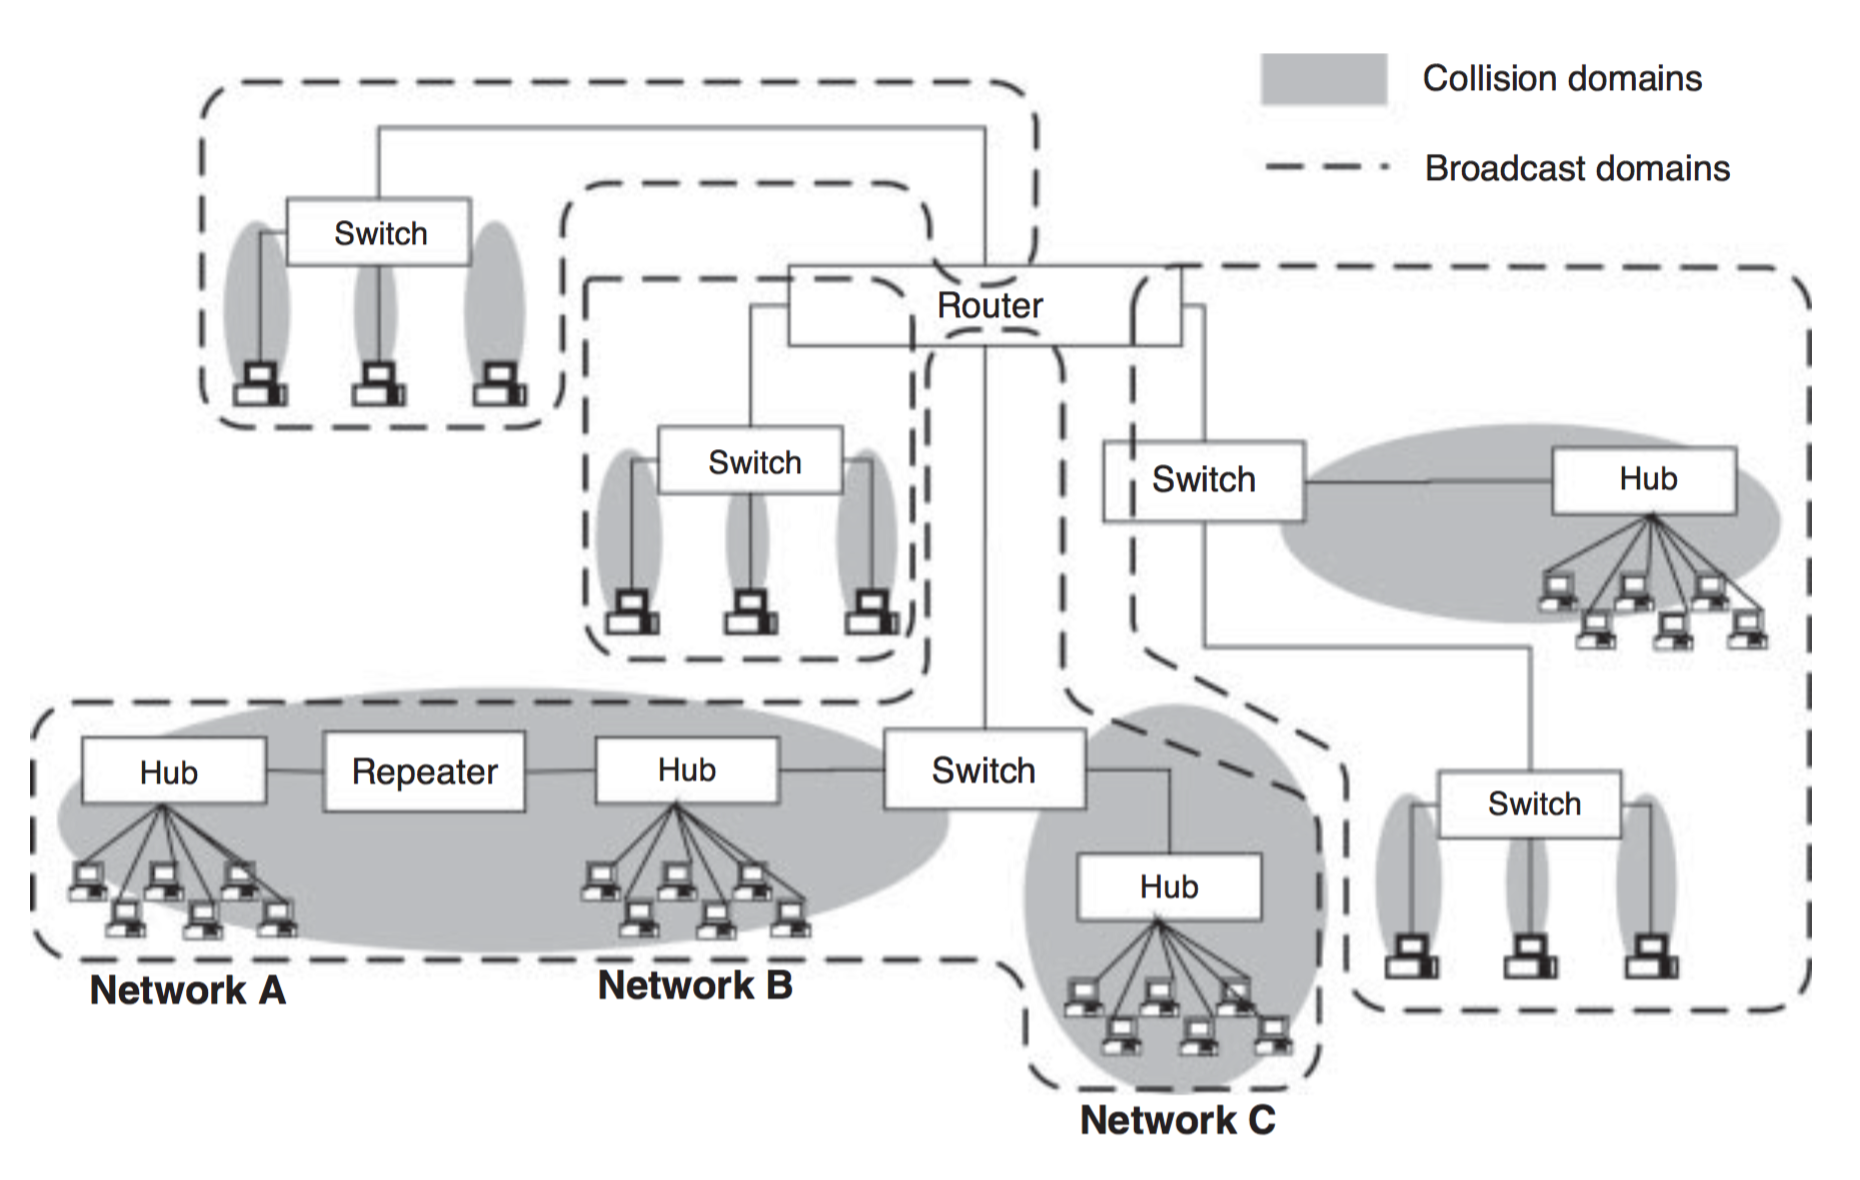
\includegraphics[scale=0.340]{imgs/lan.png}
	\caption{LAN Ethernet} \label{fig:lan}
\end{figure}
I Bridge limitano i domini di collisione mentre i Router limitano entrambi i domini. In Figura \ref{fig:lan} è mostrato come un pacchetto inviato dalla rete A può collidere con uno della rete B, ma non con uno inviato da C.
\subsubsection{Wireless}
IEEE 802.11 definisce un insieme di standard per le Wireless LAN (WLAN). L'interoperabilità dei dispositivi IEEE 802.11 è certificata dalla Wi-Fi Alliance. Una LAN Wireless è costituita dai seguenti componenti:
\begin{itemize}
	\item\emph{Station}: descrive qualsiasi dispositivo che comunica tramite una rete WLAN, ad esempio, un computer portatile, o cellulari che supportano WiFi. Nelle reti Ad-hoc questi dispositivi possono comunicare tra loro, creando una rete mesh (vedi Figura \ref{fig:bss}a). L'insieme di station che formano la rete Ad-hoc è chiamato Independent Basic Service Set (IBSS);
	\item\emph{Access Point (AP)}: consente ad una stazione di comunicare con un altra facendo da tramite. Necessita il doppio della larghezza di banda necessaria se la stessa comunicazione avvenisse direttamente tra le stazioni comunicanti. Gli AP rendono il sistema scalabile e consentono la connessione cablata con altre reti. In presenza di AP (vedi Figura \ref{fig:bss}b) l'insieme delle station è chiamato Infrastructure BSS;
	\item\emph{Distribution System}: interconnette Infrastructure BSS attraverso gli AP, come mostrato nella Figura \ref{fig:ds}. Facilita la comunicazione tra gli AP, l'inoltro del traffico da un BSS ad un altro ed il movimento di mobile station tra BSS. Un insieme di Infrastructure BSS è chiamato Extended Service Set (ESS).
\end{itemize}
La famiglia di reti LAN Wireless 802.11 utilizza il protocollo CSMA/CA per l'accesso al mezzo trasmissivo. Sono noti vari standard identificati da 802.11a/b/g/n/ac con variazioni a livello fisico. Una tipica applicazione di 802.11 nelle Smart Grid è mostrata in Figura \ref{fig:802_sg}.
\vspace{20pt}
\begin{figure}[h]
	\centering
	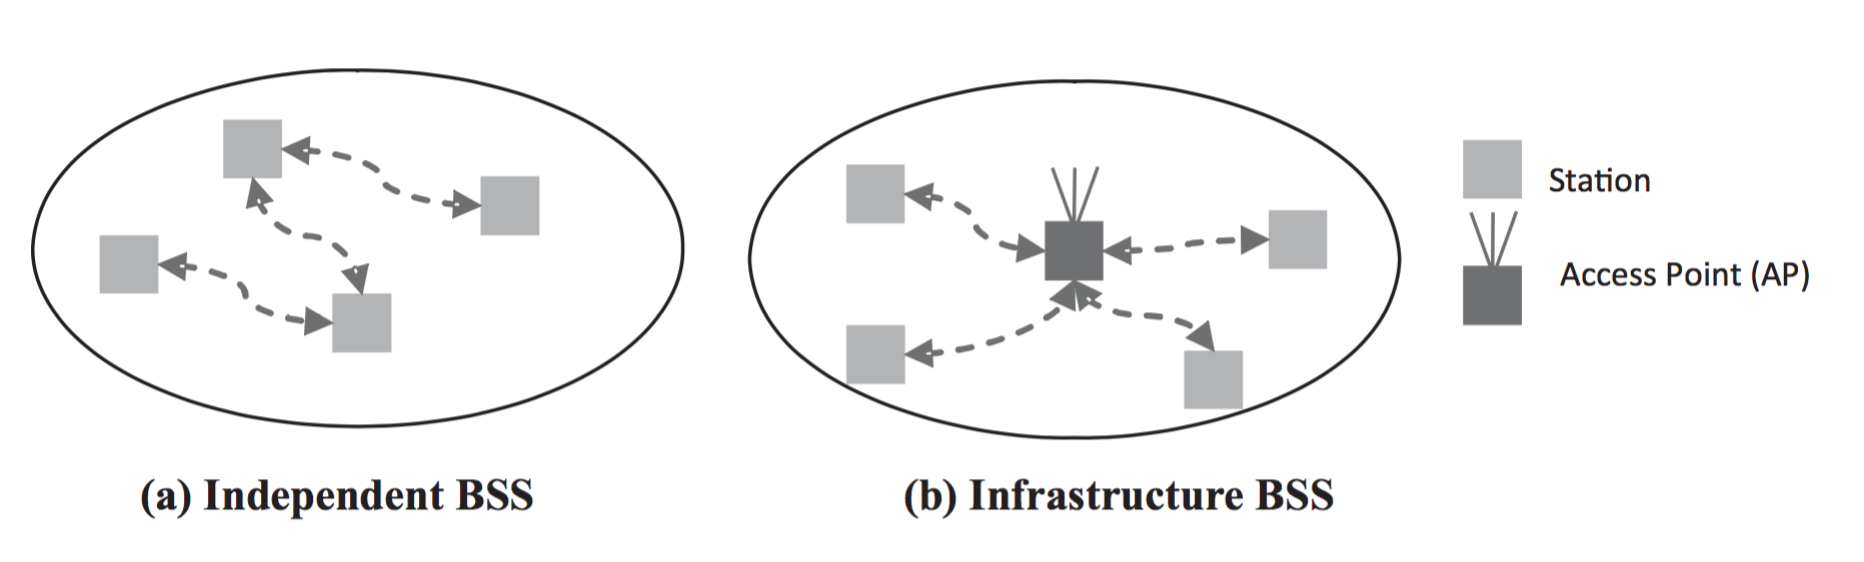
\includegraphics[scale=0.250]{imgs/bss.png}
	\caption{Architetture BSS di WLAN} \label{fig:bss}
\end{figure}
\vspace{30pt}
\begin{figure}[h]
	\centering
	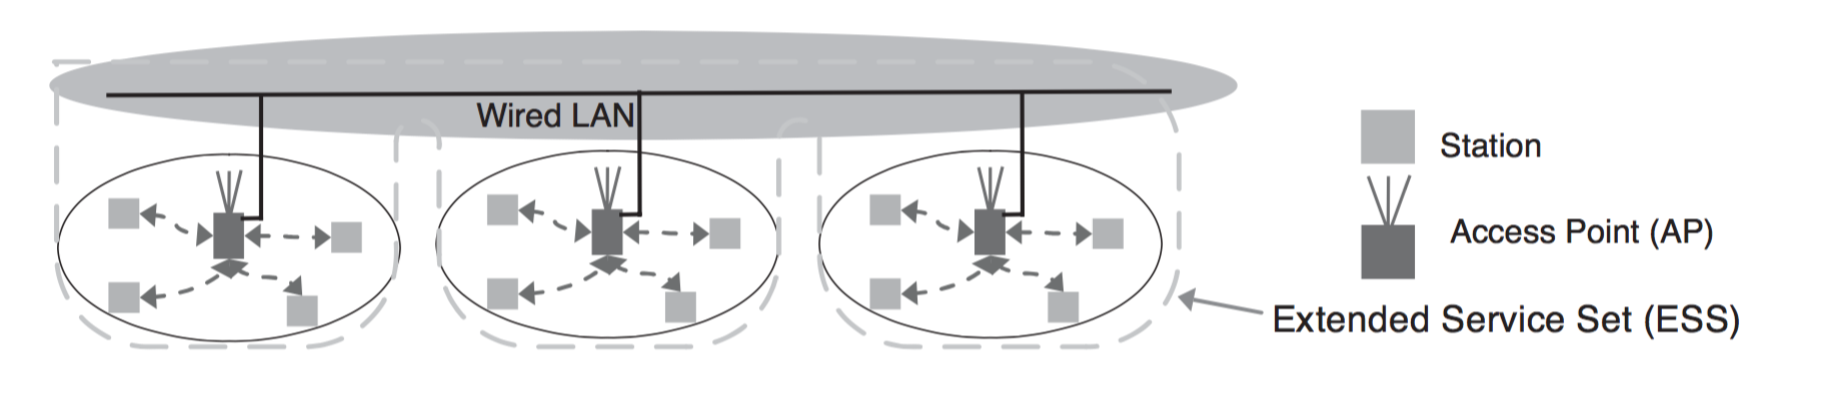
\includegraphics[scale=0.450]{imgs/ds.png}
	\caption{Distribution System} \label{fig:ds}
\end{figure}
\begin{figure}[h]
	\centering
	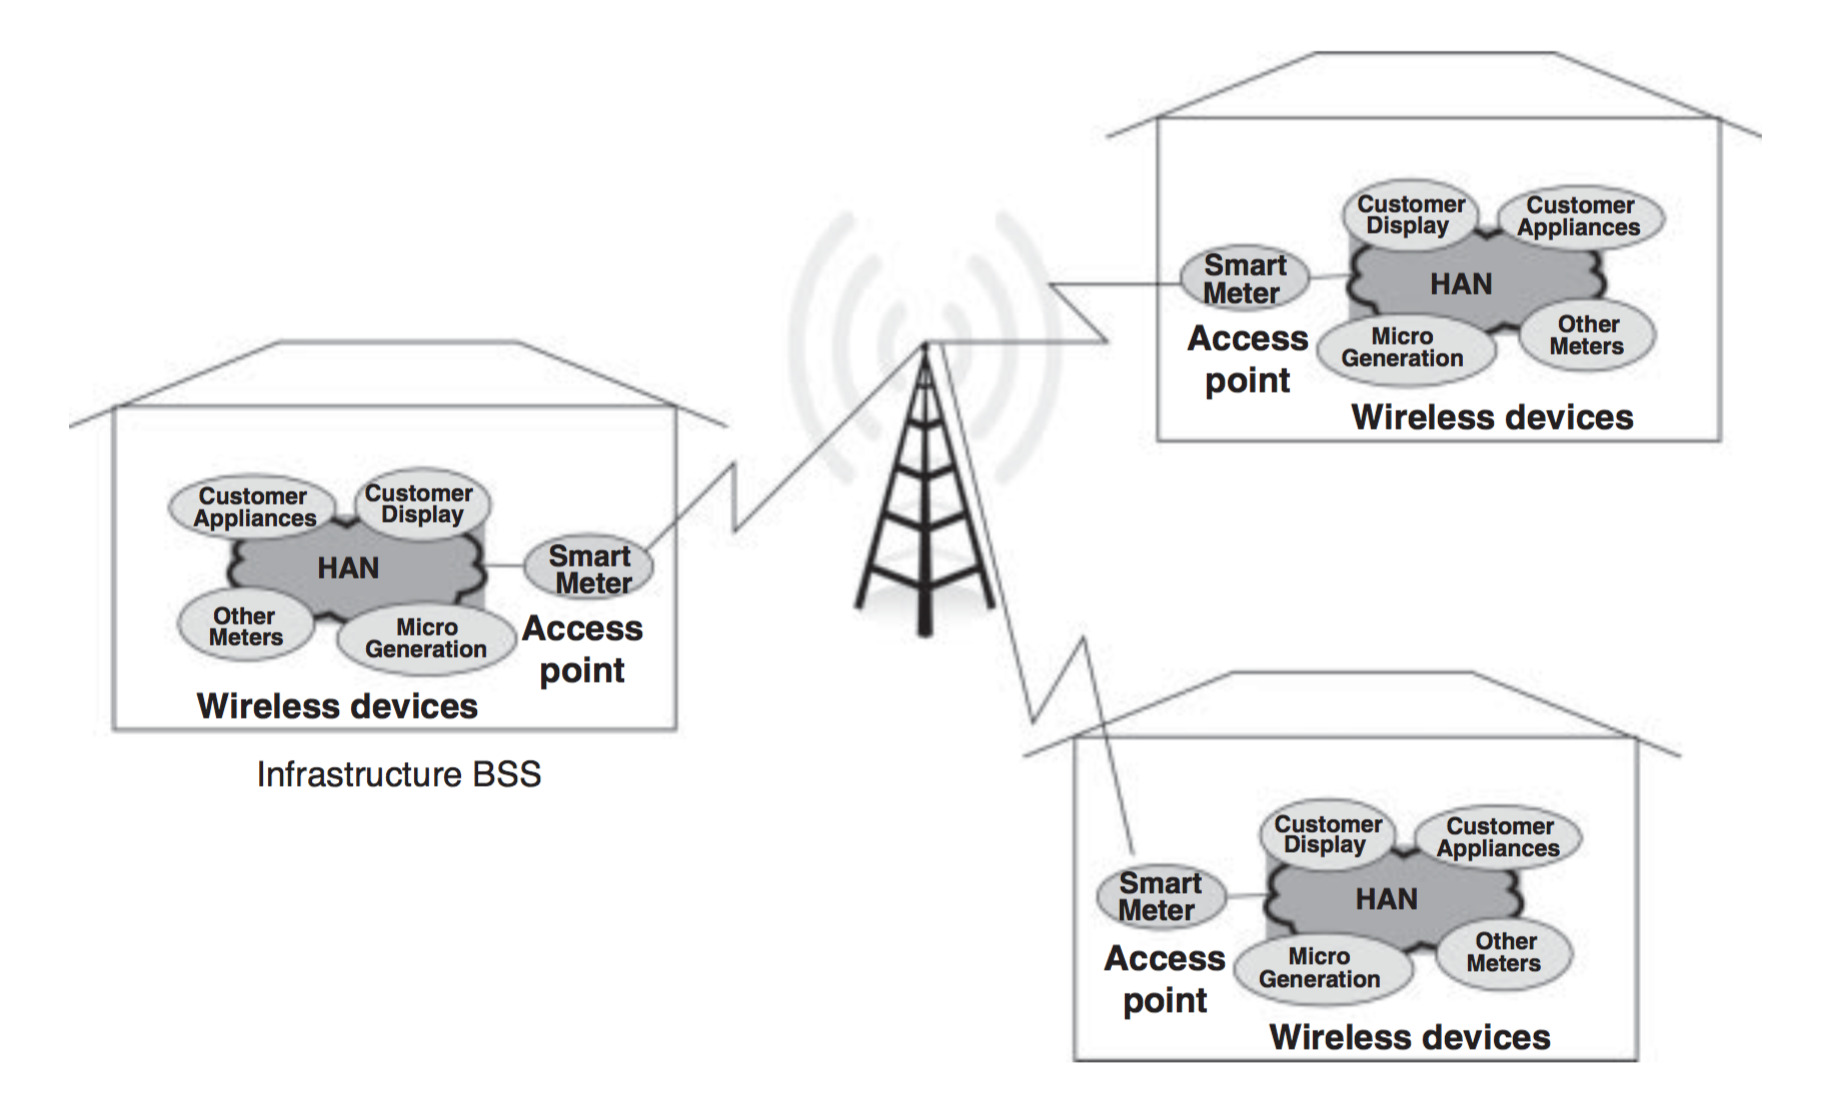
\includegraphics[scale=0.350]{imgs/80211smartgrid.png}
	\caption{Applicazione di WLAN 802.11 in una Smart Grid} \label{fig:802_sg}
\end{figure}\newpage
\subsubsection{Bluetooth}
Bluetooth, definito dallo standard IEEE 802.15.1, è una tecnologia LAN wireless progettata per collegare i dispositivi mobili o fissi con bassi consumi, un corto raggio d'azione (fino a 100 metri di copertura) e un basso costo di produzione per i dispositivi compatibili. 
Bluetooth definisce due architetture di rete denominate Piconet e Scatternet. La Piconet è costituita da un dispositivo \emph{Master} e fino a sette dispositivi \emph{Slave}. Altri dispositivi possono sincronizzarsi col Master ma non possono partecipare alla comunicazione. Si dice che tali dispositivi sono in un parked state. Un device in parked state può passare in active state se il numero di Slave della Piconet è inferiore a sette. Le Piconet possono essere interconnesse attraverso un Bridge che può essere Slave per una Piconet e Master per un'altra oppure Slave per due Piconet che sono interconnesse come in Figura \ref{fig:bt}a e \ref{fig:bt}b. Un insieme di Piconet forma una Scatternet.\newpage
Per il trasferimento dei dati è possibile creare due tipi di collegamenti bluetooth:
\begin{itemize}
		\item Synchronous Connection Orientated (SCO) link
		\item Asynchronous Connectionless Link (ACL)
\end{itemize}
SCO è utilizzato quando la consegna tempestiva è più importante della consegna senza errori mentre ACL è utilizzato nel caso inverso.
\begin{figure}[h]
	\centering
	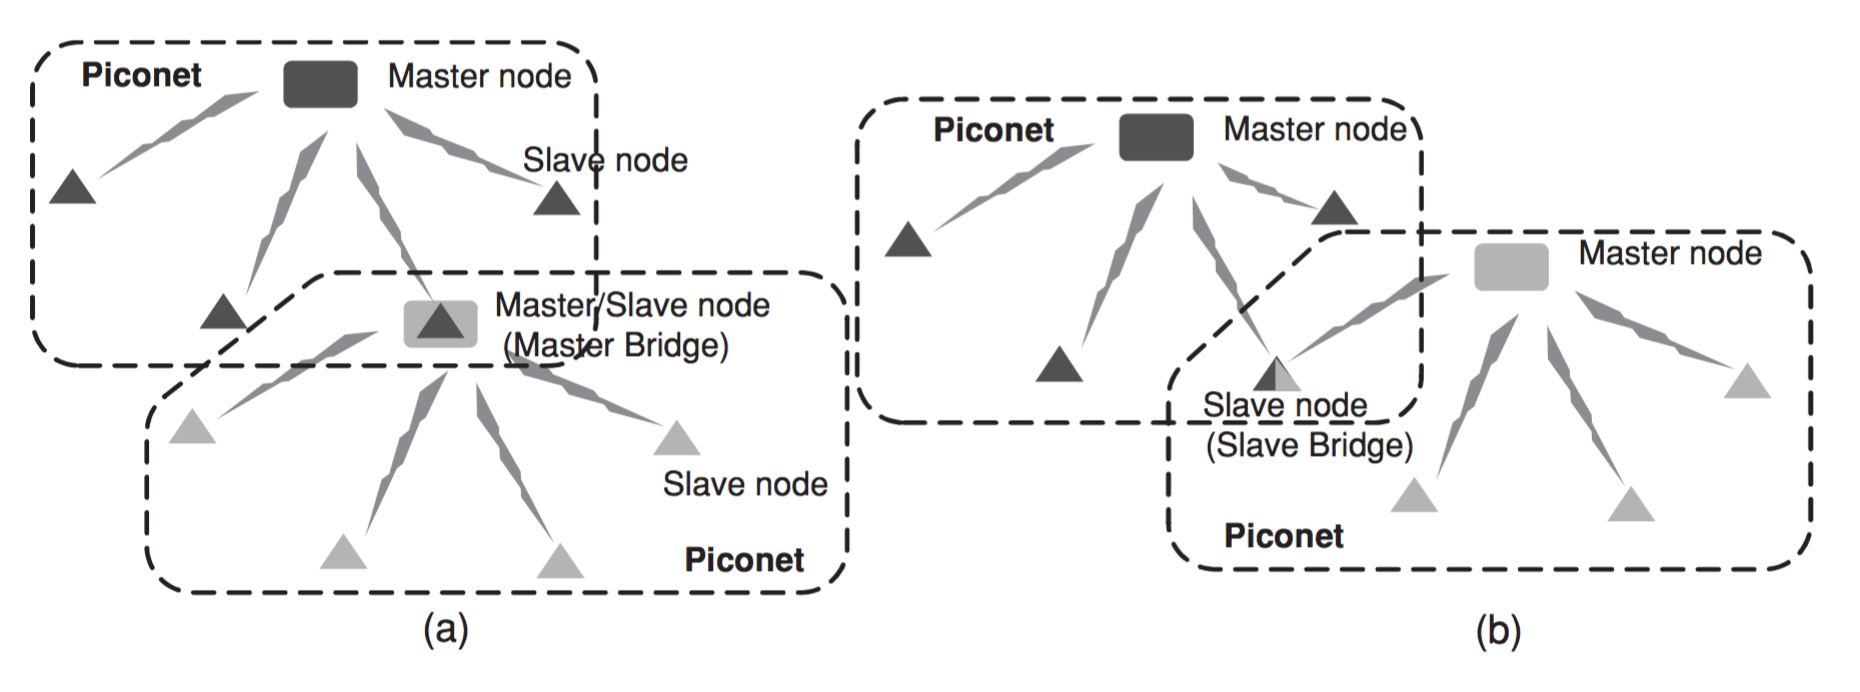
\includegraphics[scale=0.350]{imgs/bt.png}
	\caption{Piconet e Scatternet} \label{fig:bt}
\end{figure}
\subsubsection{ZigBee and 6LoWPAN}
ZigBee e 6LoWPAN sono due tecnologie di comunicazione basate su IEEE 802.15.4 per Wireless Personal Area Network (WPAN) dato il basso consumo, l'alta flessibilità ed i basso costi. L'architettura protocollare di un device ZigBee è mostrata nella Figura \ref{fig:zbprot} in cui i due strati inferiori sono definiti da IEEE 802.15.4. Application Support e Network Layer per la rete ZigBee sono definiti dalla ZigBee Alliance\cite{zb}.
\begin{figure}[h]
	\centering
	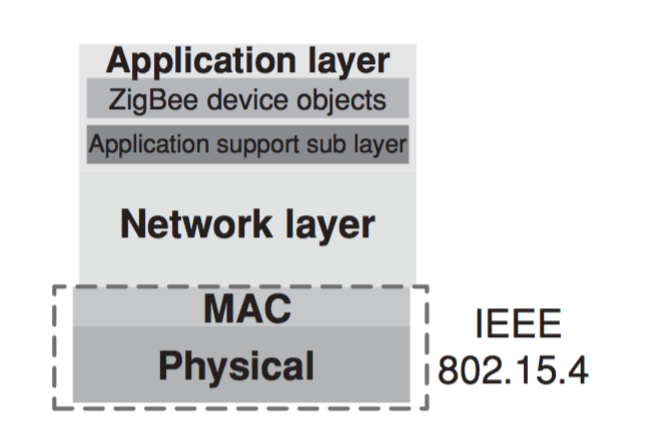
\includegraphics[scale=0.400]{imgs/zbprot.png}
	\caption{Architettura Protocollare di ZigBee} \label{fig:zbprot}
\end{figure}\newpage
Un device ZigBee può essere un Full Function Device (FFD) o un Reduced Function Device (RFD). Una rete avrà almeno un FFD, che fungerà da coordinatore della WPAN. Il FFD può funzionare in tre modalità: coordinatore, router o device. Un RFD può funzionare solo come device. Un FFD può interagire sia con un altro FFD che con un RFD, mentre un RFD può parlare solo con un FFD.
La tecnologia ZigBee è considerata come una buona opzione per il metering e per la gestione dell'energia ideale in implementazioni Smart Grid data la semplicità, mobilità, robustezza e i bassi costi di sviluppo. Offre anche programmi di pricing e monitoraggio del sistema real-time. ZigBee presenta però alcuni vincoli relativi alle basse capacità di elaborazione, alla piccola dimensione della memoria e alle interferenze tra i vari apparecchi che condividono lo stesso mezzo trasmissivo. Tali problematiche, in condizioni di rumore, aumentano la possibilità di danneggiare il canale di comunicazione a causa delle interferenze. Schemi di interference detection/avoidance e protocolli di routing energy-efficient estendono il tempo di vita della rete e forniscono una performance di rete affidabile e ad alta efficienza dal punto di vista energetico.
\newline\newline
6LoWPAN è un protocollo che consente l'invio e la ricezione di pacchetti IPv6 nelle reti basate su IEEE 802.15.4. In tale protocollo è stato inserito un Adaptation Layer (vedi Figura \ref{fig:6pan}) per il collegamento tra lo strato MAC e il Network Layer IPv6.
%Il concetto 6LoWPAN nasce dall'idea che "il protocollo Internet potrebbe e dovrebbe essere applicato anche ai dispositivi più piccoli, e che i dispositivi a bassa potenza e con capacità di elaborazione limitate dovrebbero essere in grado di far parte dell' Internet of Things".
\begin{figure}[h]
	\centering
	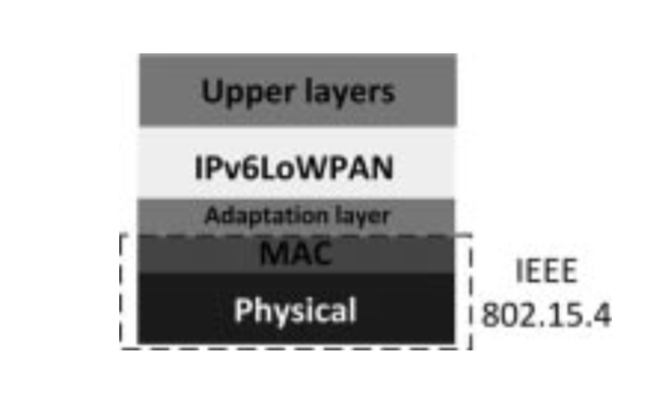
\includegraphics[scale=0.400]{imgs/6pan.png}
	\caption{Architettura di rete 6LoWPAN} \label{fig:6pan}
\end{figure}
\\
Quando un RFD in una 6LoWPAN vuole inviare un pacchetto di dati ad un dispositivo che si trova al di fuori del dominio 6LoWPAN, invia inizialmente il pacchetto ad un FFD nella stessa WPAN. Il FFD che agisce da router, inoltrerà il pacchetto dati di hop in hop fino al gateway 6LoWPAN. Il gateway 6LoWPAN potrà quindi inoltrare il pacchetto al dispositivo di destinazione utilizzando l'indirizzo IP (vedi Figura \ref{fig:6pancom}).
\begin{figure}[h]
	\centering
	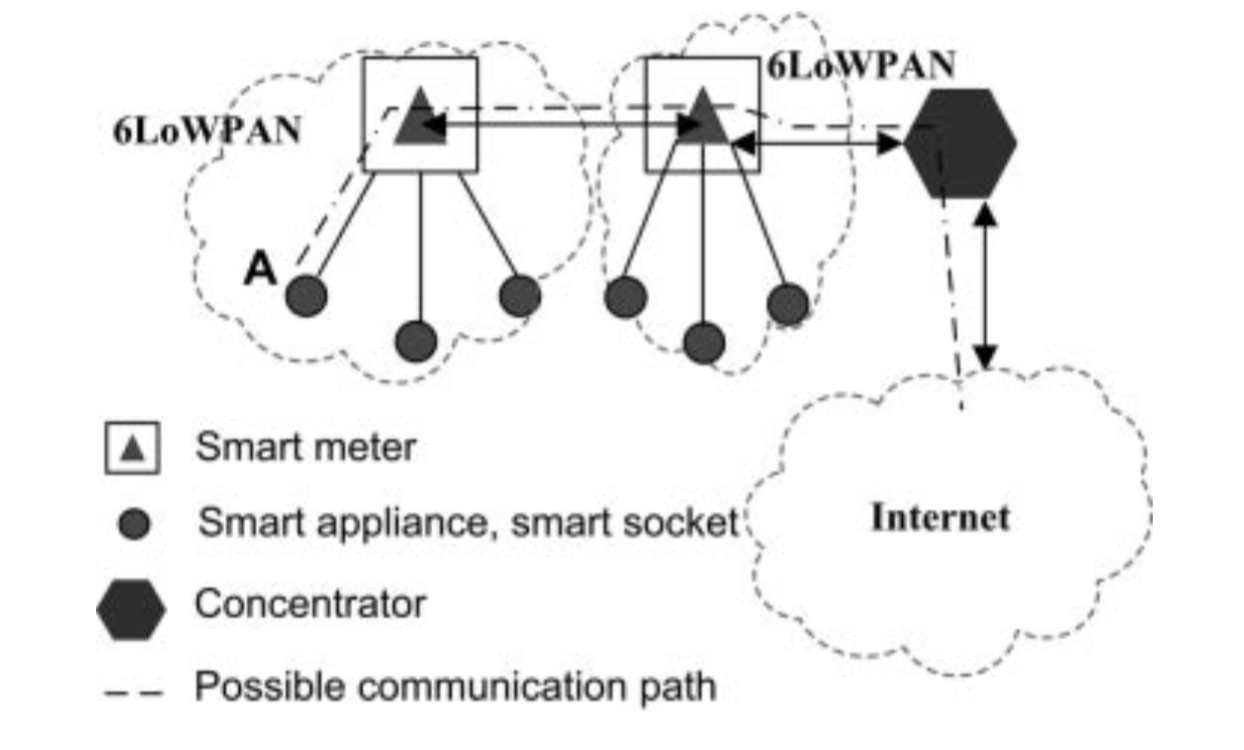
\includegraphics[scale=0.450]{imgs/6pancom.png}
	\caption{Comunicazione in una rete 6LoWPAN} \label{fig:6pancom}
\end{figure}
\subsubsection{WiMax}
Worldwide Interoperability for Microwave Access (WiMAX) è una tecnologia wireless conforme allo standard IEEE 802.16. Risulta superiore rispetto a Wi-Fi per velocità di trasmissione e range di copertura delle celle, per cui è adatto ad una trasmissione sia di tipo urbano che rurale. Inoltre, implementa diverse tecniche di crittografia, sicurezza ed autenticazione. WiMAX è una tecnologia in grado di integrarsi con quelle presenti, soddisfacendo diverse specifiche imposte da una tipica Smart Grid tra cui la massima accessibilità ed interoperabilità, tempi di latenza inferiori ai 50ms e larghezza di banda di 5MHz. Fornisce sia connettività fissa che mobile usando una tecnica chiamata Orthogonal Frequency Division Multiple Access (OFDMA). Una tipica rete WiMax è mostrata in Figura \ref{fig:wim}. La copertura di WiMax si estende fino ai 50 km con una velocità di trasmissione dati pari a 75 Mbps per i collegamenti fissi e fino a 15 Mbps per le connessioni mobili. È ottimizzato per supportare dispositivi mobili fino ad una velocità di 10 km/h. Anche se supporta veicoli in movimento fino a 120 km/h, le sue prestazioni degradano con l'aumentare della velocità del veicolo\cite{wimax}.
\begin{figure}[h]
	\centering
	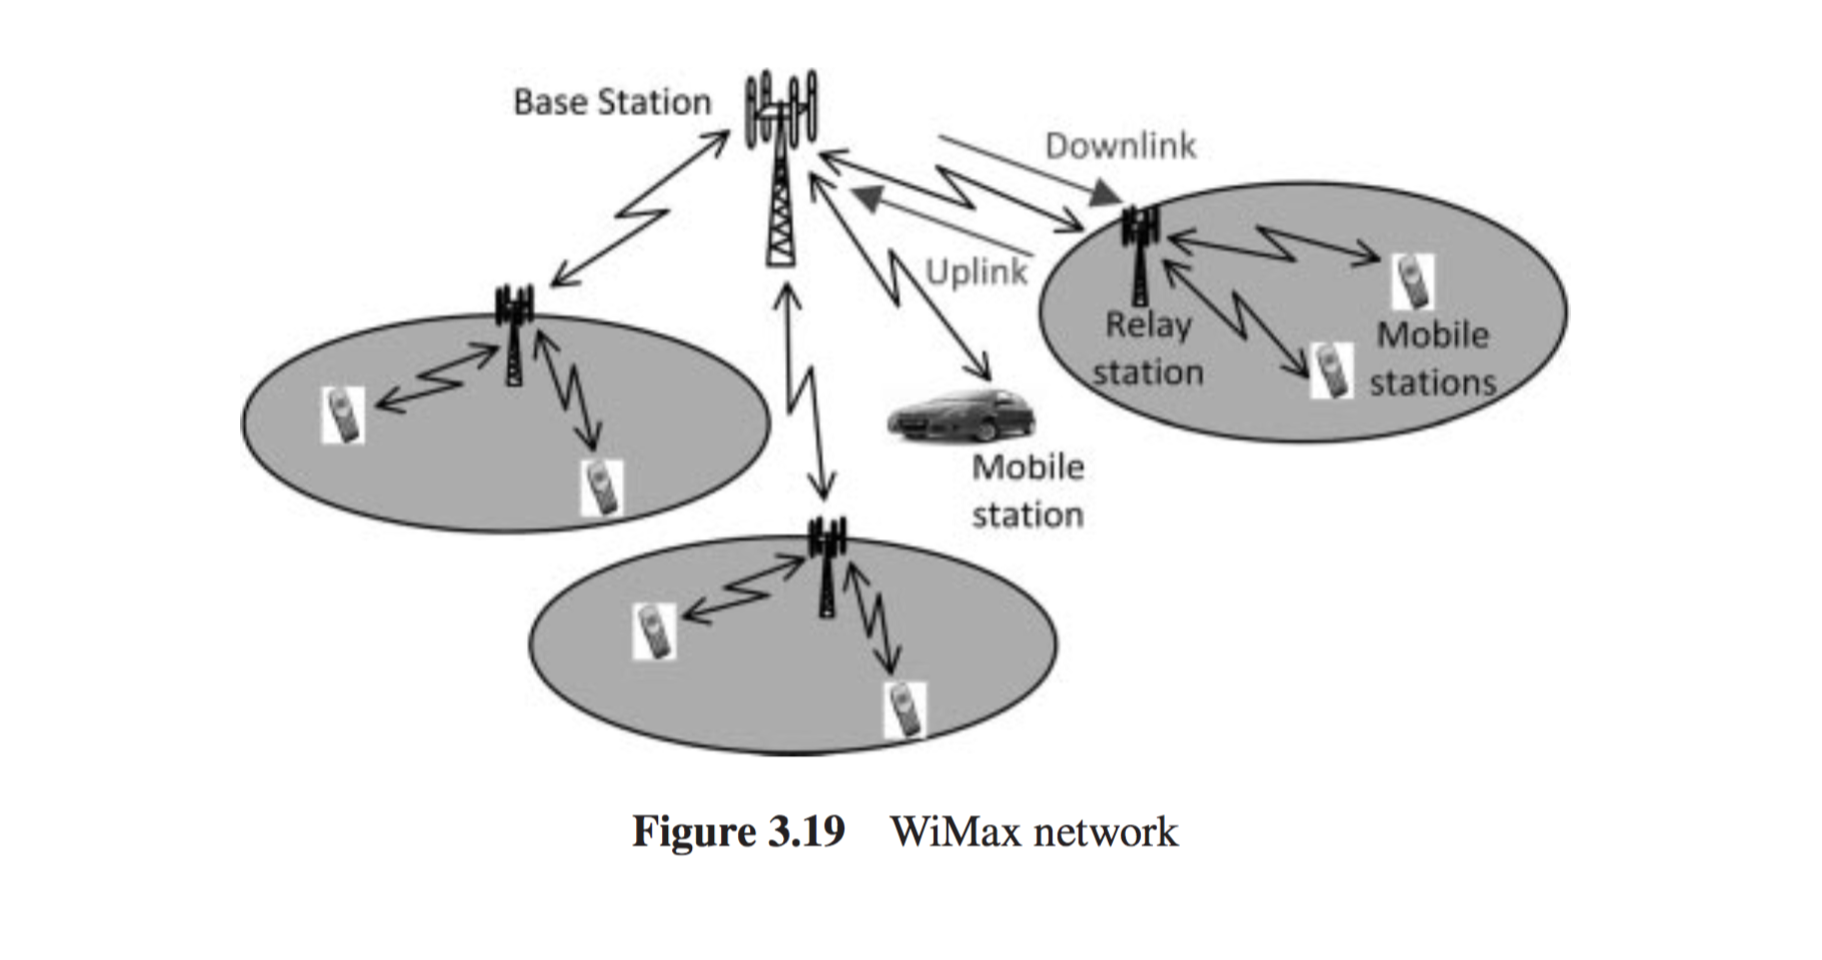
\includegraphics[scale=0.350]{imgs/wim.png}
	\caption{Una rete WiMax} \label{fig:wim}
\end{figure}
\newpage
\subsection{Power line}
La Power Line Communication (PLC) rappresenta una delle tecnologie di rete proposte per la trasmissione in ambiente Smart Grid in quanto l'infrastruttura esistente ne riduce i costi di installazione. Se, da un lato non è richiesta la realizzazione di nuove strutture, da un altro lato vi è un limite dovuto alla presenza di disturbi che possono corrompere le informazioni, non garantendo più la continuità del servizio. PLC trasporta i dati utilizzando i conduttori e le linee elettriche esistenti. Fornisce servizi di comunicazione per Automatic Meter Reading (AMR), AMI e HAN ma anche l'accesso ad internet all'utente finale. In una tipica rete PLC, gli smart meter sono collegati al data concentrator (che colleziona le informazioni ricevute dai vari meter) attraverso power line e i dati vengono trasferiti al data center tramite tecnologie di rete cellulare. La tecnologia PLC è infatti scelta per la comunicazione tra gli smart meter e il data concentrator, mentre la tecnologia GPRS è utilizzata per trasferire i dati dal concentrator al data center.\newline\newline
L'ENEL, nota azienda multinazionale produttrice e distributrice di energia elettrica, ha scelto la tecnologia PLC per trasferire i dati degli smart meter al data concentrator più vicino e la tecnologia GSM per inviare i dati al data center.
La topologia di rete, il numero/tipo dei dispositivi collegati e la distanza trasmettitore/ricevitore compromettono la qualità del segnale.
\newpage
Le sensibilità di PLC ai disturbi e alla qualità del segnale sono gli svantaggi che rendono la tecnologia non adatta alla trasmissione dei dati. Tuttavia, ci sono state alcune soluzioni ibride in cui la tecnologia PLC si combina con altre, ad esempio, GPRS o GSM, per fornire una connettività non possibile generalmente con PLC.\newline\newline
Inizialmente, la velocità di trasmissione in questo tipo di reti era molto limitata, fino a pochi kbps. Successivamente, grazie al progresso tecnologico e con l'introduzione di broadband PLC (BB-PLC), un'applicazione della tecnologia PLC a banda larga che fornisce l'accesso a Internet tramite linee elettriche ordinarie, la velocità di trasmissione ha raggiunto anche i 200 Mbps. Sono utilizzate tre tecnologie di comunicazione che prendono il nome di \emph{narrowband transmission}, \emph{spread-spectrum transmission} e \emph{DSP-processed narrowband transmission}. La Figura \ref{fig:vs_plc} mostra alcuni vantaggi e svantaggi relativi a PLC in ambito Smart Grid. Tra gli standard e i protocolli maggiormente utilizzati troviamo IEEE P1901 e HomePlug.\vspace{20pt}
\begin{figure}[h]
	\centering
	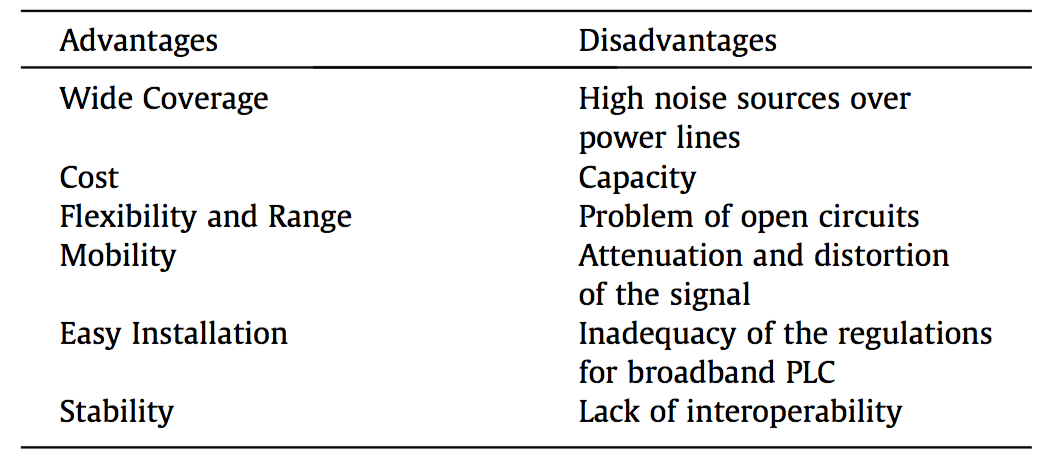
\includegraphics[scale=0.500]{imgs/vs_plc.png}
	\caption{Vantaggi e Svantaggi di PLC in ambito Smart Grid} \label{fig:vs_plc}
\end{figure}
\newpage
\subsubsection{IEEE P1901}
Il gruppo IEEE P1901 è stato formato nel 2005 con lo scopo di sviluppare una tecnologia per la trasmissione di voce o dati che utilizzasse la rete di alimentazione elettrica come mezzo trasmissivo. Lo standard permette una comunicazione ad altà velocità tra i device che prendono il nome di BPL (Broadband over Power Line). Lo standard utilizza frequenze inferiori a 100 MHz ed è di supporto ai device BPL utilizzati per i collegamenti first-mile/last-mile così come quelli utilizzati nelle reti LAN all'interno di edifici. Inoltre, tali device possono essere utilizzati all'interno di smart energy application, autoveicoli e in altre applicazioni per la distribuzione dei dati.
\subsubsection{HomePlug}
HomePlug è una tecnologia broadband non standardizzata e specificata dalla HomePlug Powerline Alliance, i cui membri sono le principali aziende nel settore della comunicazione e dell'energia. Il protocollo gestisce vari sottocanali suddividendo la larghezza di banda disponibile. La velocità di trasmissione varia da 1 a 14 Mbps e i nodi sono in grado di adattarsi al data rate ottimale in maniera automatica. Le collisioni sono evitate grazie al CSMA/CD. Lo standard HomePlug 1.0 per la connessione di dispositivi nelle case (1-10 Mbps) fa uso della tecnica di Orthogonal Frequency Division (OFDM), utilizzata anche da DSL, IEEE 802.11a e IEEE 802.11g. Il rumore, comune in ambiente power line, è superato per mezzo di forward error correction e data interleaving. La HomePlug Powerline Alliance ha definito ulteriori standard come HomePlug AV/AV2 che forniscono banda sufficiente per applicazioni come HDTV e VoIP, HomePlug CC e HomePlug BPL.
\section{Standard per lo scambio di informazioni}
\subsection{Standard per Smart Meter}
Gli smart meter possono essere utilizzati in vari modi portando a differenti requisiti dal punto di vista del sistema di comunicazione. Con Automated Meter Reading (AMR) si richiede una trasmissione occasionale dei dati energetici registrati (circa una volta al mese), viceversa con  Advanced Metering Infrastructure (AMI) si richiedono frequenti comunicazioni bidirezionali (ad esempio ogni 30 minuti). ISO/IEC 62056 e ANSI C12.22 sono due famiglie di standard che descrivono sistemi di comunicazione per gli smart meter. ISO/IEC 62056 definisce Transport e Application Layer per lo smart metering nell'ambito di una serie di specifiche chiamate COSEM (Companion Specification for Energy Metering). ANSI C12.22 (vedi Figura \ref{fig:arch_c1222}) specifica l'invio e la ricezione dei dati registrati da e verso sistemi esterni ed è possibile utilizzarlo su qualsiasi rete di comunicazione.
\begin{figure}[h]
	\centering
	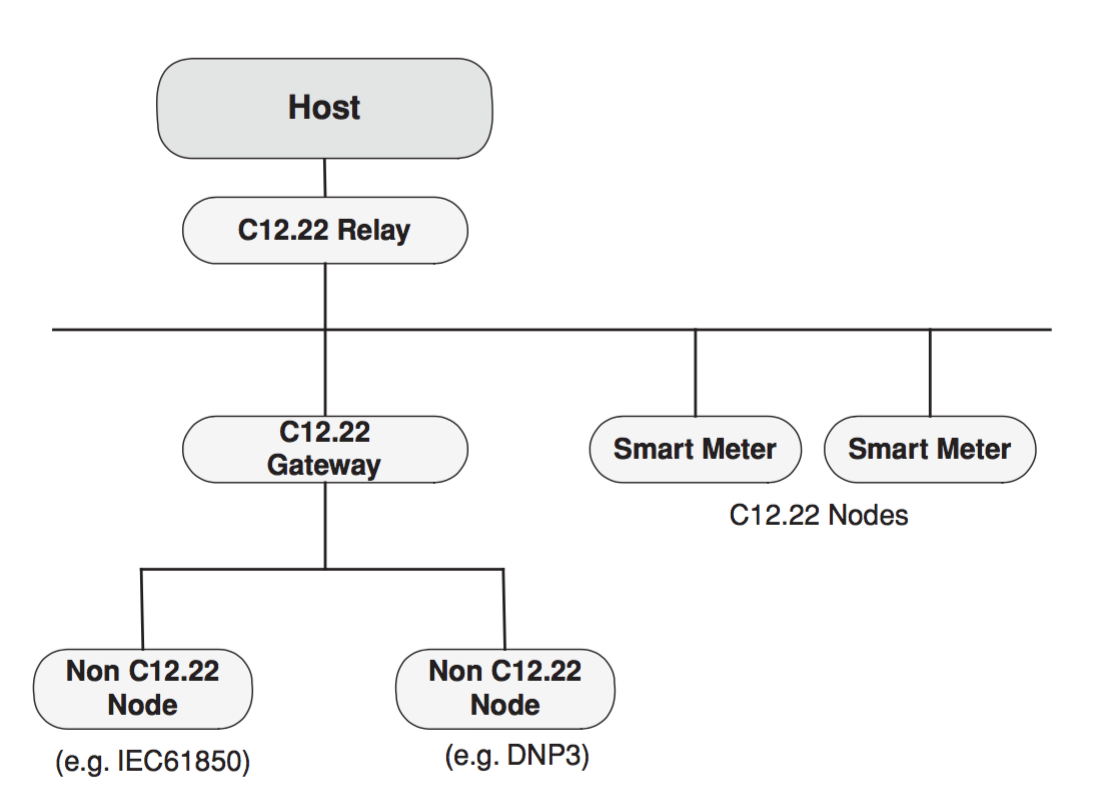
\includegraphics[scale=0.400]{imgs/arch_c1222.png}
	\caption{Architettura ANSI C12.22} \label{fig:arch_c1222}
\end{figure}
\subsection{Modbus}
Modbus è un protocollo di messaggistica che risiede nell'Application Layer e consente la comunicazione tra i dispositivi collegati su diversi bus e reti. Può essere implementato tramite Ethernet o utilizzando la trasmissione seriale asincrona su EIA 232, EIA 422, EIA 485 e fibra ottica. Di questi, l'applicazione più comune è Modbus su EIA485. La Figura \ref{fig:modbus} mostra come l'Application Layer Modbus è connesso agli altri layer del modello OSI.
Modbus su EIA 485 è ampiamente utilizzato nell'automazione delle sottostazioni. La comunicazione è avviata dal Master con una query. Il Master è l'unico che può inviare query destinate al singolo Slave o di broadcast. Uno Slave monitora continuamente la rete riconoscendo solo le query destinate ad esso. All'arrivo di una query, lo Slave eseguirà un'azione o risponderà. Tra i problemi del protocollo spiccano il limitato supporto alle varie tipologie di dati e la non garanzia di sicurezza.
\begin{figure}[h]
	\centering
	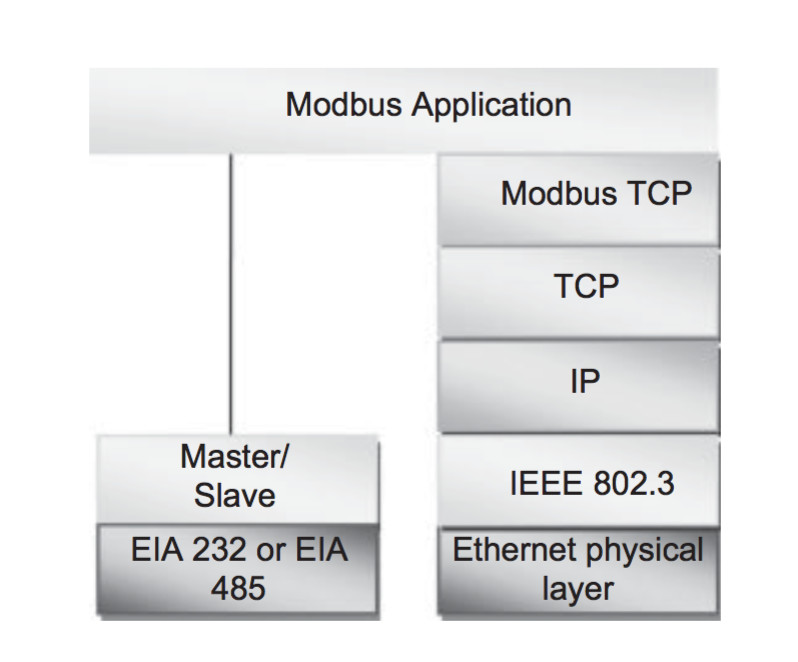
\includegraphics[scale=0.500]{imgs/modbus.png}
	\caption{Modbus stack} \label{fig:modbus}
\end{figure}
\newpage
\subsection{DNP3}
DNP3 è un insieme di protocolli di comunicazione utilizzato tra i componenti nei sistemi di automazione. DNP3 gioca un ruolo fondamentale all'interno dei sistemi SCADA, utilizzato dalle SCADA Master Station (conosciute anche come \emph{centri di controllo}) per comunicare con le Remote Terminal Unit (RTU) e/o gli Intelligent Electronic Device (IED). DNP3 è stato recentemente adottato come standard IEEE 1815-2010\cite{dnp}. Lo User Layer DNP prende input analogici/binari e da in output segnali analogici/binari. Un Master DNP3 invia richieste e le stazioni Slave DNP3 rispondono. Uno Slave DNP3 può anche trasmettere un messaggio senza aver ricevuto alcuna richiesta. Il Physical Layer DNP3 utilizza alcuni tra i più noti protocolli di comunicazione seriali come EIA 232 o EIA 485.
\newline\newline
Poiché in applicazioni Smart Grid generalmente si presume l'accesso di terze parti alla stessa rete e all'infrastruttura sottostante basata su protocollo IP, un passo in avanti è stato quello che ha portato all'aggiunta di un'autenticazione sicura al protocollo DNP3. Alcuni vendor supportano la crittografia via \textbf{bump-in-the-wire} (cioè con dispositivi esterni che cifrano e decifrano i dati agli estremi del canale di comunicazione) per le comunicazioni seriali e tramite VPN per le reti IP. Uno dei metodi bump-in-the-wire più popolari è noto come \emph{AGA-12} (American Gas Association).
\subsection{ISO/IEC 61850}
ISO/IEC 61850 è uno standard per la progettazione dei sistemi di automazione per le sottostazioni elettriche. E' una sovrastruttura che coordina e gestisce protocolli e tecnologie esistenti garantendo l'interoperabilità. Generalmente, questi protocolli girano su reti TCP/IP o LAN con switch Ethernet molto performanti per rispondere ai requisiti stringenti dei dispositivi, che necessitano di tempi di risposta inferiori a 4-5 millisecondi.\newline\newline
I principali vantaggi dello standard ISO/IEC 61850:
\begin{itemize}
	\item Coordina la complessità di tante unità indipendenti;
	\item Si integra con i sistemi preinstallati in rete;
	\item E' scalabile e facilita l'integrazione di apparati diversi;
	\item Si basa il più possibile su standard esistenti;
	\item E' aperto e supporta i \emph{self descriptive device} eliminando problemi di configurazione manuale;
	\item Si basa sui \emph{data object} e standardizzazione degli elementi tipici di una rete elettrica;
	\item Permette di ottenere alte prestazioni di multicast;
	\item E' estensibile e flessibile in modo da adattarsi rapidamente alla configurazione del sistema.
\end{itemize}
\newpage
La struttura dello standard ISO/IEC 61850\cite{iec61850} è mostrata in Figura \ref{fig:iec61850}.
\begin{figure}[h]
	\centering
	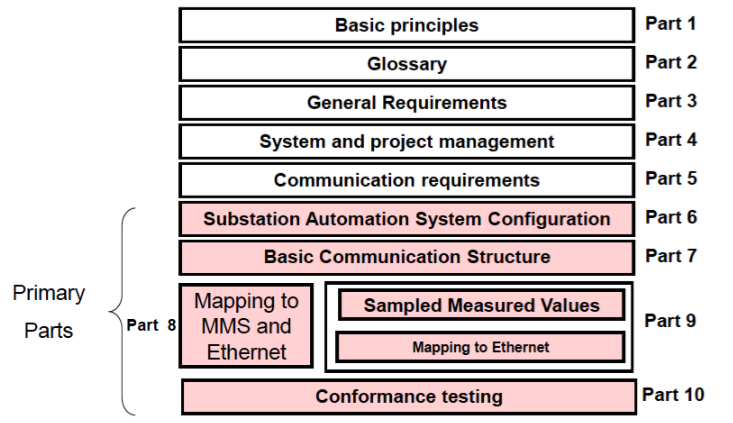
\includegraphics[scale=0.400]{imgs/iec61850.png}
	\caption{Struttura dello standard ISO/IEC 61850} \label{fig:iec61850}
\end{figure}\\
ISO/IEC 61850 suddivide ogni sottostazione in tre livelli\cite{iec61850} chiamati \emph{Station Level}, \emph{Bay Level} e \emph{Process Level}. La suddivisione dei livelli è mostrata in Figura \ref{fig:61850ls}.

\begin{figure}[h]
	\centering
	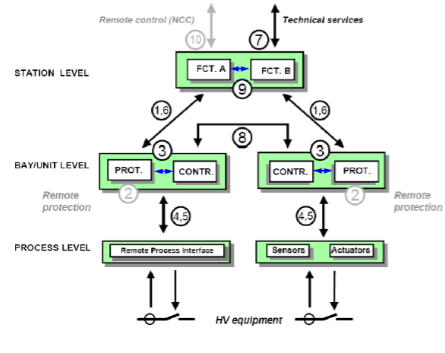
\includegraphics[scale=0.400]{imgs/61850ls.png}
	\caption{Livelli di una sottostazione} \label{fig:61850ls}
\end{figure}

Il protocollo identifica le funzioni e le caratteristiche dei dispositivi fisici che si modellano in uno o più dispositivi logici. I dispositivi logici sono a loro volta suddivisi in nodi logici che sono in relazione tra loro in base a \emph{data} e \emph{data attribute} (vedi Figura \ref{fig:iec61850ln}).
\begin{figure}[h]
	\centering
	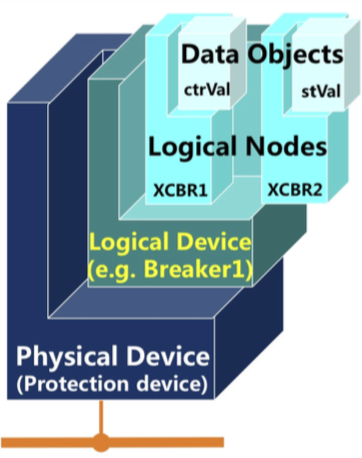
\includegraphics[scale=0.350]{imgs/iec61850ln.png}
	\caption{Device Model ISO/IEC 61850} \label{fig:iec61850ln}
\end{figure}
\newpage
Come mostrato in Figura \ref{fig:iec61850ds}a, un device model considera inizialmente un physical device. Tale modello consente ad un singolo dispositivo fisico di agire da gateway di informazioni per più dispositivi. Successivamente vengono specificati i logical device all'interno di tale dispositivo. Ogni logical device contiene uno o più logical node, logicamente correlati ad una funzione della stazione. I logical node sono definiti da gruppi di data object e relativi servizi, ognuno modellato secondo gli schemi definiti dalle \textbf{Common Data Classes} (CDC).\newline
\begin{figure}[h]
	\centering
	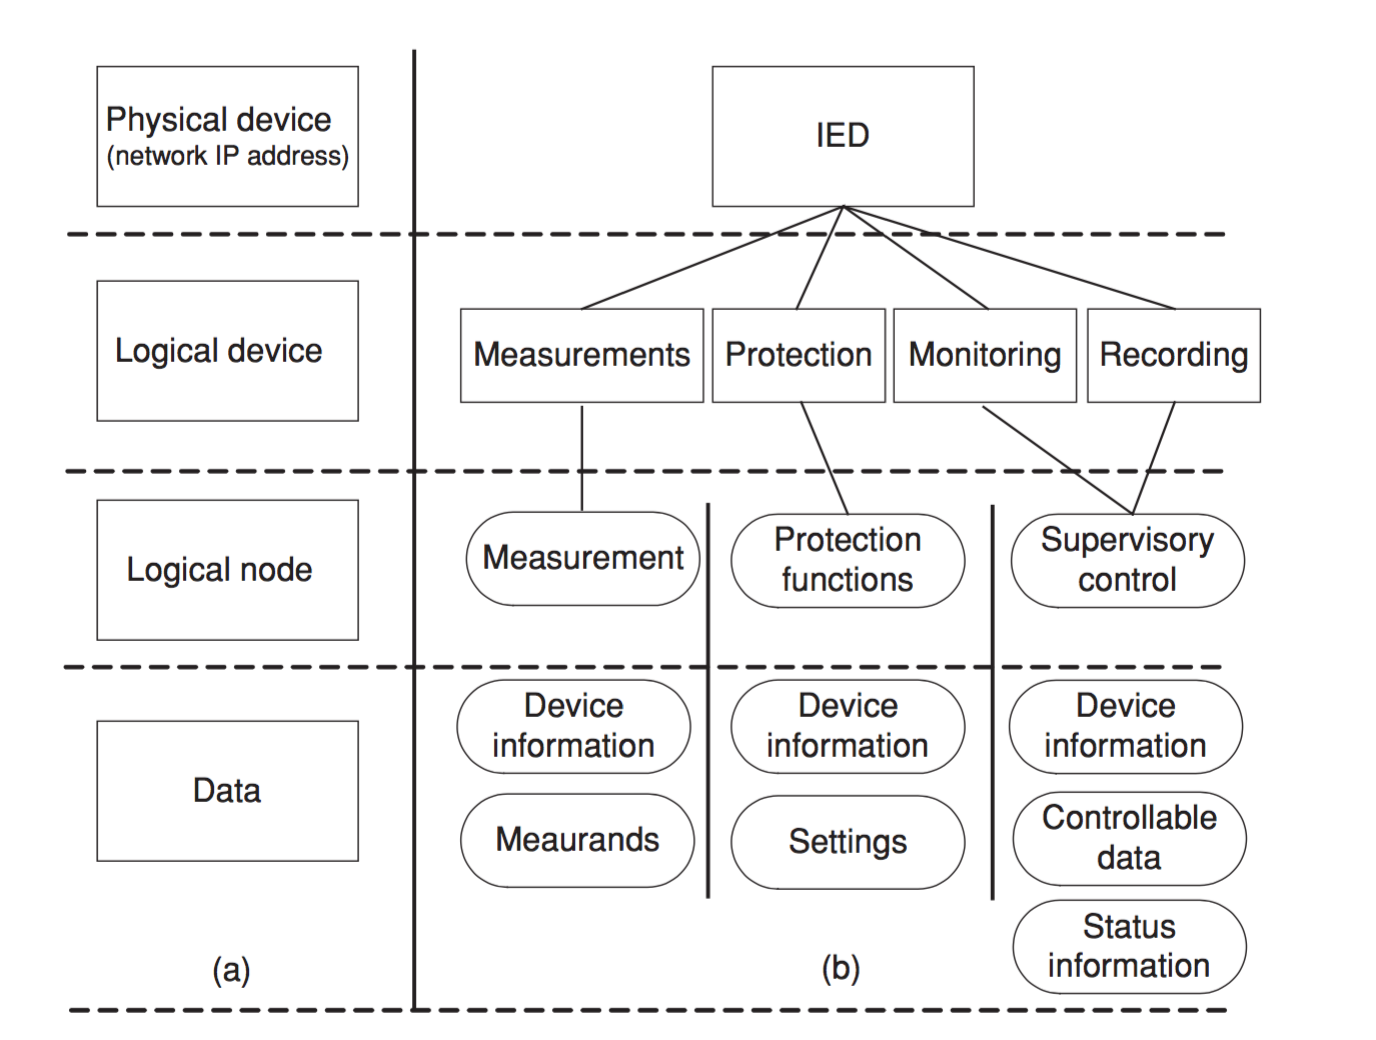
\includegraphics[scale=0.350]{imgs/iec61850ds.png}
	\caption{ISO/IEC 61850 data structure} \label{fig:iec61850ds}
\end{figure}\newpage
La Figura \ref{fig:name_obj} mostra un esempio di nome per un oggetto in un formato standard. Utilizzando tale formato si è in grado di indicare le informazioni relative allo status o alla posizione di un dispositivo. I logical node sono identificati con nomi definiti dallo standard in cui la prima lettera indica l'attinenza (e.g. A controllo automatico, M misura, X switchgear, etc).
\begin{figure}[h]
	\centering
	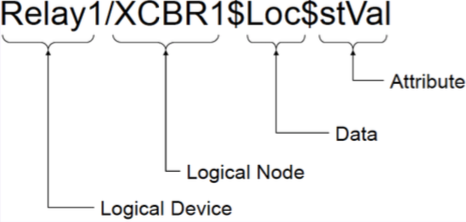
\includegraphics[scale=0.350]{imgs/name_obj.png}
	\caption{Struttura del nome di un oggetto} \label{fig:name_obj}
\end{figure}
\newline
L'ISO/IEC 61850 si basa sulla specifica degli \emph{oggetti} e dei \emph{servizi astratti} di comunicazione che permettono di scrivere un'applicazione indipendentemente dai protocolli tradizionali. Si definisce quindi un modello che prende il nome di Abstract Communication Service Interface (ACSI) che definisce l'insieme dei servizi e le risposte a quei servizi che rendono gli IED uguali dal punto di vista della rete. Inoltre, tale modello interpreta i dati e gli attributi dei vari elementi garantendone l'interoperabilità. Gli oggetti e i servizi definiti dall'ACSI vengono implementati attraverso il protocollo ISO-9560 Manufacturing Message Specification (MMS). Si tratta di un protocollo flessibile in grado di supportare funzioni complesse e la logica a oggetti ACSI. Tale protocollo definisce i messaggi di comunicazione tra i vari centri di controllo oppure tra le stazioni e i centri di controllo.\newline\newline
Il concetto di astrazione e standardizzazione presuppone l'utilizzo di un linguaggio comune di configurazione. L'ISO/IEC 61850 si serve di un linguaggio basato su \emph{XML} chiamato \emph{Substation Configuration Language} (SCL). Grazie all'utilizzo di un linguaggio standard è possibile garantire l'interoperabilità tra gli IED che usano diversi protocolli, permettere una configurazione automatica dei dispositivi, ridurre la presenza di errori dovuti all'intervento umano nella gestione degli IED e consentire maggiore trasportabilità facendo in modo che ogni IED, che supporta ISO/IEC 61850, presenti un file SCL che ne definisce la configurazione. Nella Figura \ref{fig:iec61850ds}b è mostrato un esempio di IED.\newpage
Gli elementi fondamentali del modello di una sottostazione sono elencati di seguito (vedi Figura \ref{fig:arch_iec61850}):
\begin{itemize}
	\item\textbf{Merge Unit}: a livello di processo, i dati raccolti da sensori ottici, elettronici, da TV e TA, sui valori di tensione e corrente o sullo status dei componenti, sono recuperati dalle Merge Unit (MU). In genere, sono situate in corrispondenza del centro di controllo;
	\item\textbf{Intelligent Electronic Device}: gli IED che supportano ISO/IEC 61850 comunicano attraverso le MU e un process bus Ethernet a 10 Gbps;
	\item\textbf{Wrapper ISO/IEC 61850}: gli IED che non supportano il protocollo ISO/IEC 61850 utilizzano un Wrapper;
	\item\textbf{Process Bus e Station Bus}: le MU comunicano con il Bay Level attraverso un process bus mentre tutti i nodi logici (IED) comunicano attraverso un bus Ethernet a 100 Mbps;
	\item\textbf{Gateway e Internet}: diverse sottostazioni comunicano tra loro attraverso la rete Internet. Un Gateway permette di collegarsi alla rete e accedere alle informazioni da un centro di controllo o da remoto seguendo una procedura che garantisce la robustezza e sicurezza del sistema.
\end{itemize}

\begin{figure}[h]
	\centering
	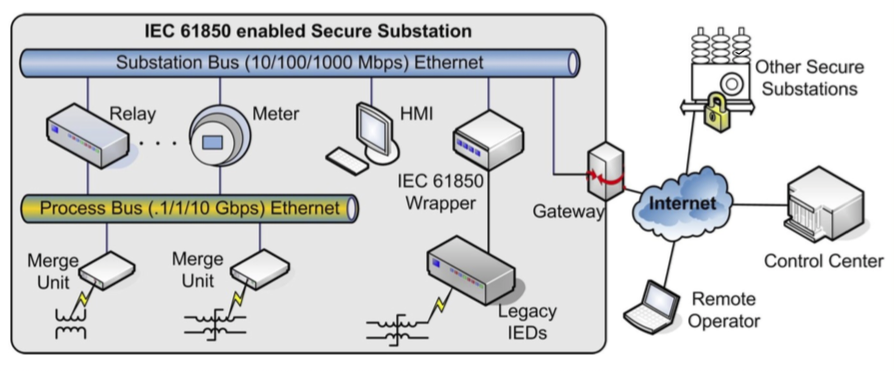
\includegraphics[scale=0.450]{imgs/arch_iec61850.png}
	\caption{Architettura del sistema con lo standard ISO/IEC 61850} \label{fig:arch_iec61850}
\end{figure}
\newpage
Lo standard ISO/IEC 61850 si serve dei seguenti strumenti per la gestione delle informazioni (vedi Figura \ref{fig:tools_iec61850}):
\begin{itemize}
	\item Generic Substation Event (GSE);
	\begin{itemize}
		\item Generic Object Oriented Substation Event (GOOSE);
		\item Generic Substation State Event (GSSE).
	\end{itemize}
	\item Sampled Measured Values (SMV);
	\item Time Synchronization;
	\item Report e Logging.
\end{itemize}
\begin{figure}[h]
	\centering
	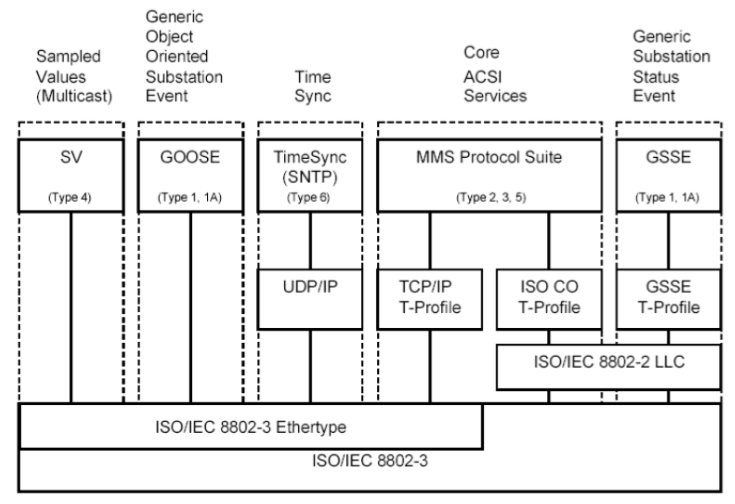
\includegraphics[scale=0.350]{imgs/tools_iec61850.png}
	\caption{Tools di ISO/IEC 618504} \label{fig:tools_iec61850}
\end{figure}
\textbf{GSE} è un protocollo che fornisce uno strumento veloce ed affidabile per la segnalazione di \emph{eventi} all'interno della sottostazione. Le caratteristiche principali sono il servizio multicast/broadcast con modello di comunicazione publish/subscribe. I messaggi sono trasmessi in formato binario. GSE prevede due modelli di servizio che prendono il nome di GOOSE e GSSE.\newline\newline
\textbf{GOOSE} è stato progettato per essere \emph{brand indipendent}. Utilizza Virtual LAN, stabilendo più network virtuali sulla stessa rete fisica e determinando livelli di priorità per i messaggi, consentendone anche la ritrasmissione (un identificativo indica se il messaggio è nuovo o ritrasmesso).\newpage
\textbf{GSSE} è utilizzato per lo scambio di informazioni sui soli cambiamenti di stato. In questo caso i messaggi sono costituiti da una serie di bit che rappresentano liste di stati. GSSE necessita un tempo di trasmissione maggiore se confrontato con GOOSE.
\newline\newline
\textbf{SMV} è un protocollo per lo scambio di dati e la trasmissione di misure prodotte dai trasduttori delle sottostazioni: permette lo scambio di segnali tra gli IED. Prevede due metodi di comunicazione:
\begin{itemize}
	\item\emph{SV over Serial Unidirectional Multidrop Point-to-Point fixed link}: Sistema di comunicazione unidirezionale che specifica una serie di dataset (tensioni trifase, correnti trifase, etc). I valori analogici vengono codificati a 16 bit;
	\item\emph{SV over Ethernet}: Versione più generica e flessibile di SV che fornisce la possibilità di definire dataset con valori di diversa dimensione e tipo, configurabili dall'utente grazie all'utilizzo di SCL. Utilizza un modello di comunicazione publish/subscribe con possibilità di multi-casting.
\end{itemize}
\textbf{Time Synchronization} è un servizio di sincronizzazione dei clock fondamentale per applicazioni real-time. Utilizza un subset di Network Time Protocol (NTP) con riferimento allo Universal Coordinated Time (UTC). NTP è il protocollo tipicamente utilizzato per sincronizzare i clock di computer collegati ad Internet e in LAN.\newline\newline
\textbf{Report} è lo strumento che permette di memorizzare i cambiamenti dei dati e degli attributi relativi ai nodi logici. Genera dataset contenenti attributi di interesse e richiede ai nodi logici l'invio delle informazioni riguardanti le variazioni nel sistema.\newline\newline
\textbf{Log} è la registrazione degli eventi relativi ad un dispositivo. I log sono registrati in un server e, a differenza dei Report, i dispositivi logici creano al loro interno un database di eventi senza inviarne notifica.\newline\newline
Tra i limiti di ISO/IEC 61850 si evidenziano i costi elevati per l'installazione dei server e dei dispositivi atti alla gestione dei dati ma anche  complessità dal punto di vista dell'architettura. ISO/IEC 61850 è affiancato da ISO/IEC 62351 che garantisce la sicurezza e specifica i requisiti tecnici che devono essere rispettati dai fornitori.
\newpage
\section{Standard per la sicurezza}
Gli standard per la sicurezza informatica sono di recente invenzione e fondamentali data la grande mole di informazioni sensibili memorizzate sui computer che sono collegati ad Internet. Inoltre, molte attività che prima erano condotte manualmente, oggi sono svolte dalle macchine in maniera automatica introducendo quindi un maggiore bisogno di affidabilità e di sicurezza in tali sistemi informatici. Come ampiamente discusso nel Capitolo 4, la sicurezza è un fattore importante per per gli individui che devono proteggersi dal cosiddetto furto di identità ma anche per le aziende perché devono proteggere i loro segreti industriali e le informazioni sui dati personali dei clienti.\newline\newline
I problemi relativi alla sicurezza vanno quindi dagli accessi non autorizzati a informazioni recuperate dagli smart meter, lo spegnimento dei dispositivi da parte di un attaccante così come un attacco alla Smart Grid per causare un'interruzione al passaggio di corrente. I problemi relativi alla privacy riguardano invece l’alta frequenza con cui vengono effettuate le letture per misurare il consumo energetico in quanto esse mostrano totalmente il comportamento dell’utente. In generale si cerca di aggregare le informazioni dei meter per rilevare sia frode che perdite (per esempio nel caso del gas, dove un'eventuale perdita pone un problema di sicurezza) utilizzando schemi di aggregazione \emph{privacy-friendly} in modo da mascherare i singoli consumi dei meter.
\newline\newline
Nell'ambito dei power system, esistono diversi standard che si applicano alla sicurezza delle apparecchiature all'interno delle sottostazioni e molti sono in fase di sviluppo. Per la valutazione complessiva della sicurezza, è ampiamente utilizzata la norma ISO 27001 e specifica la valutazione dei rischi e la strategia da utilizzare per lo sviluppo di un sistema di sicurezza in modo da limitarli.
\subsection{ISO/IEC 62351}
ISO/IEC 62351 è uno standard sviluppato dal WG15 facente parte della TC57 dell'organo internazionale IEC. Questo standard è stato sviluppato per gestire la sicurezza nella serie di protocolli della commissione tecnica 57, tra i quali le serie ISO/IEC 60870-5, ISO/IEC 60870-6 series, ISO/IEC 61850, ISO/IEC 61970 e ISO/IEC 61968.\newpage
Tra i diversi obiettivi di sicurezza che lo standard persegue ci sono:
\begin{itemize}
	\item Autenticazione nel processo di trasferimento di dati tramite firma digitale;
	\item Garanzia di accessi esclusivamente dopo autenticazione;
	\item Prevenzione dell'\emph{eavesdropping} (ossia intercettazioni della comunicazione non autorizzate);
	\item Prevenzione da attacchi di \emph{playback} e attacchi di  \emph{spoofing} (ovvero sostituirsi ad una controparte della comunicazione);
	\item Rilevamento delle intrusioni.
\end{itemize}
Le prime due parti di ISO/IEC 62351 comprendono la spiegazione di differenti scenari e la definizione di alcuni termini. ISO/IEC 62351 utilizza i protocolli di sicurezza esistenti, come il Transport Layer Security (TLS, \cite{tls}), utilizzato con successo in altre aree tecniche e in diverse parti dello standard. TLS offre servizi di sicurezza come la mutua autenticazione dei peer in una comunicazione (utile per contrastare attacchi  \emph{man-in-the-middle}) ma si occupa anche dell'integrità e della riservatezza dei dati comunicati. La terza parte di ISO/IEC 62351 definisce come possono essere forniti servizi di sicurezza in una  comunicazione TCP/IP based e specifica suite di cifratura. La quarta parte specifica le procedure, i miglioramenti del protocollo, e gli algoritmi atti a promuovere l'aumento dei messaggi di sicurezza trasmessi su MMS. Questa parte definisce alcune procedure relative a Transport e Application Layer, basate su TLS, in modo da proteggere le informazioni trasmesse. La quinta parte riguarda invece la comunicazione seriale in cui si vanno a definire ulteriori misure di sicurezza per proteggere l'integrità delle connessioni seriali applicando chiavi hash. Questa parte specifica quindi anche una separata gestione delle chiavi. La sesta parte di ISO/IEC 62351 si occupa dei profili di ISO/IEC 61850 per la comunicazione, non basati su TCP/IP. La settima parte è utile poichè implementa e/o estende sistemi di intrusion detection e l'ottava ed ultima parte si occupa di role-based access control.

\begin{thebibliography}{99}
\bibitem{802.3} \url{http://www.ieee802.org/minutes/2011-March/802\%20workshop/index.shtml}.
\bibitem{zb} ZigBee Specification, ZigBee Alliance, ZigBee Document 053474r17, January 2008.
\bibitem{wimax} Cudak, M. (ed.) (2010) IEEE 802.16m System Requirements, IEEE 802.16 Task Group M, January 2010, \url{http://ieee802.org/16/tgm/docs/80216m-07_002r10.pdf}.
\bibitem{dnp} IEEE Power \& Energy Society (2010) IEEE Std 1815TM-2010: IEEE Standard for Electric Power Systems Communications-Distributed Network Protocol (DNP3), June.
\bibitem{iec61850} IEC 61850 - communication networks and systems in substation: an overview of computer science.
University of Illinois at Urbana Champaign, jan. 2010.
\bibitem{tls} RFC 5246: The Transport Layer Security (TLS) Protocol, Version 1.2, T. Dierks, E Rescorla, August 2008
\end{thebibliography}